
In Experiments 1--5,
I classified cursor trajectories as either
direct movements to a response,
or reversals/changes of mind.
To do this, I fit two-sample finite mixture models
to the Maximum Deviation data from each experiment,
and from these derived Maximum Deviation cut-offs,
above which trials could be classed as reversals.

\newpage

\FloatBarrier
\section*{Experiment 1}\label{experiment-1}

\begin{figure}[ht]
  \centering
  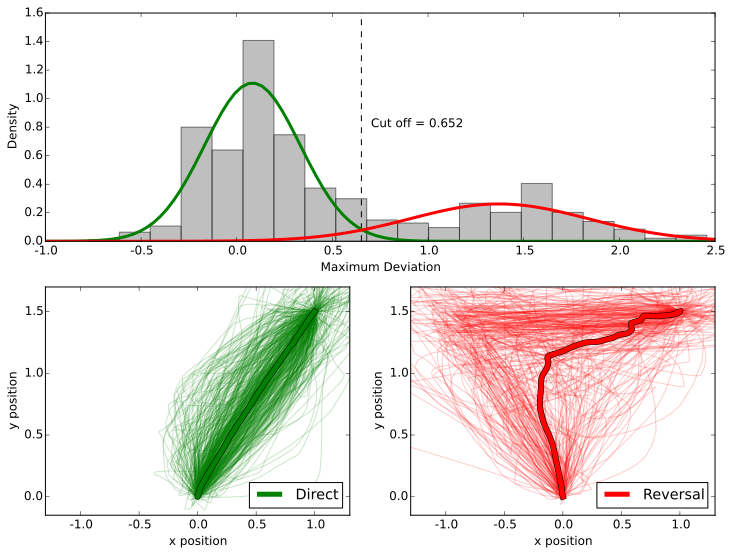
\includegraphics[width=\textwidth]{imgs/reversals/exp1-reversals}
  \caption[]{
    \label{fig:exp1-reversals}
    Trajectories classed as direct and reversals in Experiment 1.
  }
\end{figure}

Bimodality Coefficient = 0.689.
Hartigan's' D = 0.027, N = 580, p = 0.006.

\begin{table}[hp]
  \centering
  \caption[]{
    Mean and SD, and relative proportions, of the Maximum Deviation for direct and reversal trials, in Experiment 1
    \label{tab:appendix-reversals-1}
  }
  \begin{tabular}{lrr}
    \toprule
                       &   Direct &   Reversal \\
    \midrule
    Mean               &     0.08 &             1.37 \\
    Standard deviation &     0.25 &             0.46 \\
    Proportion         &    70\%    &            30\%    \\
    \bottomrule
  \end{tabular}
  
\end{table}


\newpage
\FloatBarrier
\section*{Experiment 2}\label{experiment-2}

\begin{figure}[ht]
  \centering
  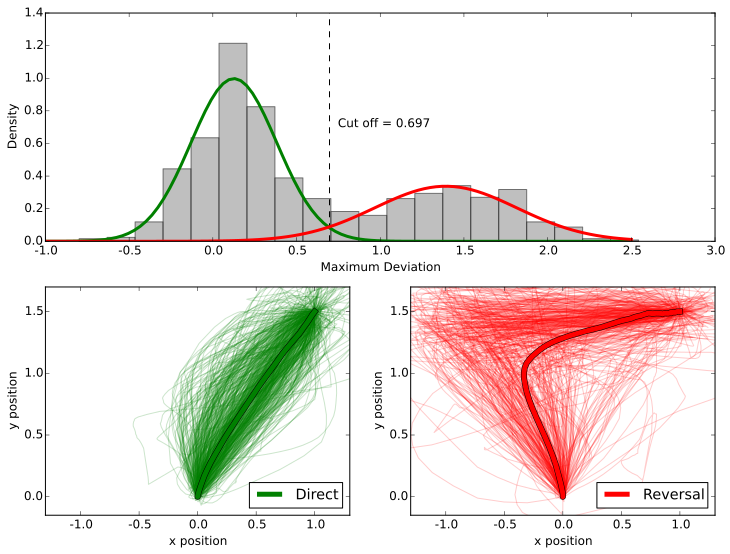
\includegraphics[width=\textwidth]{imgs/reversals/exp2-reversals}
  \caption[]{
    \label{fig:exp2-reversals}
    Trajectories classed as direct and reversals in Experiment 2.
  }
\end{figure}


Bimodality Coefficient = 0.65.
Hartigan's' D = 0.021, N = 754, p = .0182.

\begin{table}[hp]
  \centering
  \caption[]{
    Mean and SD, and relative proportions, of the Maximum Deviation for direct and reversal trials, in Experiment 2
    \label{tab:appendix-reversals-2}
  }
  \begin{tabular}{lrr}
    \toprule
    &   Direct &   Reversal \\
    \midrule
    Mean               &     0.13 &             1.39 \\
    Standard deviation &     0.26 &             0.42 \\
    Proportion         &    64\%    &            36\%    \\
    \bottomrule
  \end{tabular}
\end{table}


\newpage
\FloatBarrier
\section*{Experiment 3}\label{experiment-3}

\begin{figure}[ht]
  \centering
  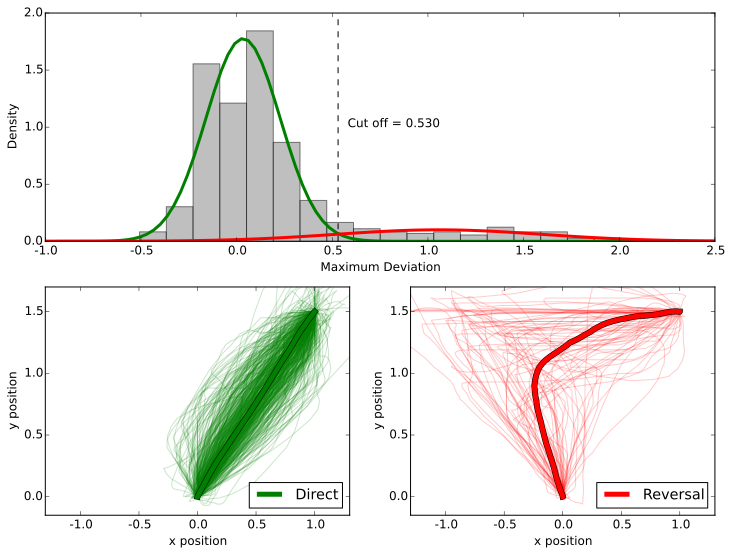
\includegraphics[width=\textwidth]{imgs/reversals/exp3-reversals}
  \caption[]{
    \label{fig:exp3-reversals}
    Trajectories classed as direct and reversals in Experiment 3
    (after data was excluded from stimulus sets for which participants
    performed poorly on the post-test check; see Chapter 4).
  }
\end{figure}


Bimodality Coefficient = 0.705.
Hartigan's' D = 0.042, N = 520, p < .0001.


\begin{table}[hp]
  \centering
  \caption[]{
    Mean and SD, and relative proportions, of the Maximum Deviation for direct and reversal trials, in Experiment 3
    \label{tab:appendix-reversals-3}
  }
  \begin{tabular}{lrr}
    \toprule
    &   Direct &   Reversal \\
    \midrule
    Mean               &     0.03 &             1.06 \\
    Standard deviation &     0.19 &             0.54 \\
    Proportion         &    86\%    &            14\%    \\
    \bottomrule
  \end{tabular}
\end{table}

\newpage
\FloatBarrier
\section*{Experiment 4}\label{experiment-4}

\begin{figure}[ht]
  \centering
  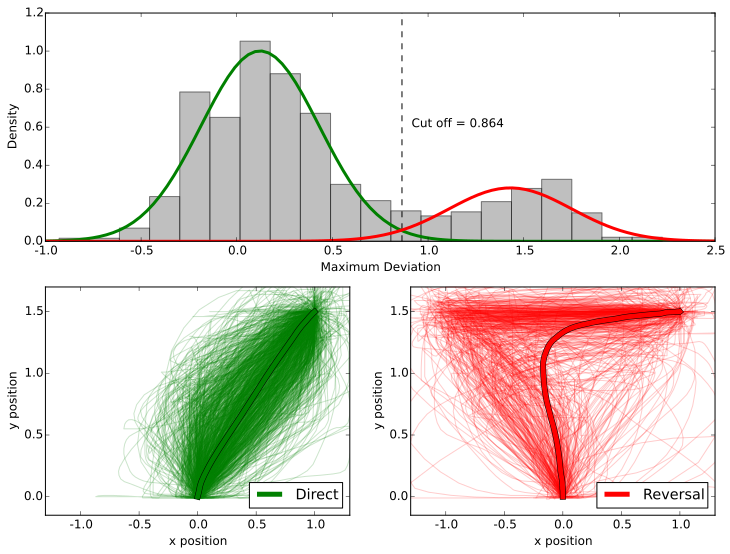
\includegraphics[width=\textwidth]{imgs/reversals/exp4-reversals}
  \caption[]{
    \label{fig:exp4-reversals}
    Trajectories classed as direct and reversals in Experiment 4.
  }
\end{figure}


Bimodality Coefficient = 0.636.
Hartigan's' D = 0.025, N = 1188, p < .0001.

\begin{table}[hp]
  \centering
  \caption[]{
    Mean and SD, and relative proportions, of the Maximum Deviation for direct and reversal trials, in Experiment 4
    \label{tab:appendix-reversals-4}
  }
  \begin{tabular}{lrr}
    \toprule
    &   Direct &   Reversal \\
    \midrule
    Mean               &     0.12 &             1.43 \\
    Standard deviation &     0.31 &             0.32 \\
    Proportion         &    77\%    &            23\%    \\
    \bottomrule
  \end{tabular}
\end{table}

\newpage
\FloatBarrier
\section*{Experiment 5}\label{experiment-5}

\begin{figure}[ht]
  \centering
  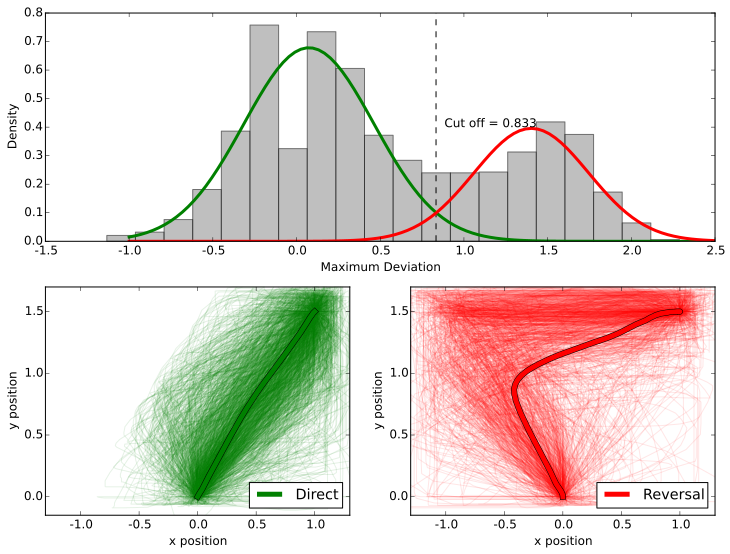
\includegraphics[width=\textwidth]{imgs/reversals/exp5-reversals}
  \caption[]{
    \label{fig:exp5-reversals}
    Trajectories classed as direct and reversals in Experiment 5.
  }
\end{figure}

Bimodality Coefficient = 0.562.
Hartigan's' D = 0.024, N = 1998, p < .0001.

\begin{table}[hp]
  \centering
  \caption[]{
    Mean and SD, and relative proportions, of the Maximum Deviation for direct and reversal trials, in Experiment 1
    \label{tab:appendix-reversals-5}
  }
  \begin{tabular}{lrr}
    \toprule
    &   Direct &   Reversal \\
    \toprule
    Mean               &     0.07 &             1.4  \\
    Standard deviation &     0.39 &             0.34 \\
    Proportion         &    66\%    &            34\%    \\
    \toprule
  \end{tabular}
\end{table}
